% !TeX program = xelatex
% !Mode:: "TeX:UTF-8"
%%  本模板推荐以下方式编译: xelatex
%%     1. 文件默认的编码为 UTF-8 对于windows,请选用支持UTF-8编码的编辑器。
%%   2. 若是模板有什么问题,请及时与我们取得联系,Email:latexstudio@qq.com。
%%   3. 可以到  https://ask.latexstudio.net 提问
%%   4. 请安装 最新版本的 TeXLive 地址:
%%   http://mirrors.ctan.org/systems/texlive/Images/texlive.iso

\documentclass[12pt,a4paper]{nmmcm}
\usepackage{ctex}
\usepackage{graphicx}
\usepackage{booktabs,colortbl}
\usepackage{xcolor}
\usepackage{tikz}
\usepackage{indentfirst}
\mcmsetup{CTeX = true,
        tcn ={\xiaowuhao 2024030125260 }, problem = C,
        sheet = true, titleinsheet = false, keywordsinsheet = true,
        titlepage = true, abstract = true}
\usepackage{xurl}
\setmainfont[
    Path=fonts/TimesNewRoman/,
    UprightFont = *-Regular,
    BoldFont = *-Bold,
    ItalicFont = *-Italic,
    BoldItalicFont = *-Bold-Italic  
]{TimesNewRoman}
\setmonofont[ 
    Path=fonts/UbuntuMono/,
    UprightFont = *-Regular,
    BoldFont = *-Bold,
    ItalicFont = *-Italic,
    BoldItalicFont = *-Bold-Italic  
]{UbuntuMono}
\usepackage{lipsum}

\usepackage{paralist}
\let\itemize\compactitem
\let\enditemize\endcompactitem
\let\enumerate\compactenum
\let\endenumerate\endcompactenum
\let\description\compactdesc
\let\enddescription\endcompactdesc

\setlength\abovedisplayskip{5pt}
\setlength\belowdisplayskip{-8pt}
\setlength{\parskip}{0.1em}

\newcommand\wordc[1]{\textbf{#1}}
\renewcommand{\appendixtocname}{附\quad录}
\renewcommand{\appendices}{\hspace{-2em}{\sanhao\HEI {\bf 附~~~录}}}
\colorlet{tableheadcolor}{gray!25} % Table header colour = 25% gray
\newcommand{\headcol}{\rowcolor{tableheadcolor}}

\title{\textcolor{red}{论文的题目(三号黑体)}}
\date{}

\usepackage[font=small,labelfont={bf,sf},tableposition=top]{caption}

% 我们团队自己的定制化操作
%%%%%%%%%%%%%%%%%%%%%%%%%%%%%%%%%%%%%%%%%%%%%%%%%%%%%%%%
\makeatletter
% 修改 section
\renewcommand\section{\@startsection{section}{1}{0pt}%
    {3.5ex plus 1ex minus .2ex}%
    {2.3ex plus .2ex}%
    {\normalfont\LARGE\bfseries}}
% 修改 subsection
\renewcommand\subsection{\@startsection{subsection}{2}{0pt}%
    {3.25ex plus 1ex minus .2ex}%
    {1.5ex plus .2ex}%
    {\normalfont\Large\bfseries}}
    % subsubsection标题的缩进
\renewcommand\subsubsection{\@startsection{subsubsection}{3}{1em}%
  {4ex plus 1ex minus .2ex}%
  {0.2ex plus .2ex}%
  {\normalfont\large\bfseries}}
\makeatother

\usepackage[backend=biber,style=gb7714-2015,gbfieldtype=true]{biblatex}
\addbibresource[location=local]{references.bib} 
%%%%%%%%%%%%%%%%%%%%%%%%%%%%%%%%%%%%%%%%%%%%%%%%%%%%%%%%%%%%

\begin{document}
\begin{abstract}
  

%abstract---------------
{\song\xiaosihao
\setlength{\parindent}{2em}\textcolor{red}{(第1段)	问题重述+简要思想:首先简要叙述所给问题的背景和动机,并分别分析每个小问题的特点(以下以三个问题为例)。根据这些特点说出自己的思想:针对于问题1,采用~$\cdots \cdots$ 的方法解决;针对问题2用~$\cdots \cdots$ 的方法解决;针对问题3用~$\cdots \cdots$ 的方法解决。}


\setlength{\parindent}{2em}\textcolor{red}{(第2段)	模型建立及求解结果:介绍思想和模型: 对于问题1我们首先建立了~$\cdots \cdots$ 模型I。首先利用~$\cdots \cdots$ ,其次计算了~$\cdots \cdots$ ,并借助~$\cdots \cdots$ 数学算法和~$\cdots \cdots$ 软件得出了~$\cdots \cdots$ 结论。}

\setlength{\parindent}{2em} \textcolor{red}{(第3段)	对于问题2我们用~$\cdots \cdots$(模型的建立与求解结果的陈述中,思想、模型、软件和结果必须描述清晰,亮点详细说明需突出。}

\setlength{\parindent}{2em}\textcolor{red}{(第4段)	对于问题3我们用~$\cdots \cdots$ (模型的建立与求解结果的陈述中,思想、模型、软件和结果必须描述清晰,亮点详细说明需突出。}

\setlength{\parindent}{2em}\textcolor{red}{(第5段)	优化结果及总结:在~$\cdots \cdots$ 条件下,针对~$\cdots \cdots$ 模型进行适当修改与优化,这种条件的改变可能来自你的一种猜想或建议。要注意合理性。此推广模型可以不深入研究,也可以没有具体结果。}
}

\begin{rmk}
    字数300$\sim $600之间,需控制在一页;摘要中必须将具体方法、模型和所得结果写出来;摘要要求“总分总”,段开头可用“针对问题1,针对问题2,针对问题3..”或者“首先,然后,其次,最后”等词语进行有逻辑的论述。摘要是重中之重,必须严格执行!
\end{rmk}







  \begin{keywords}
    {\song\xiaosihao
      \textcolor{red}{天然气水合物、资源预测、核密度估计、Kriging 插值、粒子群优化算法}}
  \end{keywords}

\end{abstract}
\maketitle
\renewcommand{\contentsname}{\centerline{\sanhao\bfseries\HEI 目\quad 录}}
%\thispagestyle{empty}
%{\song\xiaosihao
\tableofcontents
%}

\newpage
\setcounter{page}{1}
\pagestyle{fancy}
\section{问题重述}
本研究针对天然气水合物(Natural Gas Hydrate/Gas Hydrate),即通常所称的“可燃冰”,
这是一种在特定高压低温环境下与水结合形成的类冰状结晶物质。由于其外观类似冰块且能在火源接触下燃烧,
故此得名。这种物质主要分布在深海沉积物或陆地的永久冻土层中,是一种被国际能源领域高度重视的潜在清洁
能源。
在能源科学研究与勘探领域中,天然气水合物的勘探和量化评估是一项复杂且技术要求高的任务。其关键挑
战包括但不限于:资源的空间定位、量化评估、经济可行性分析以及对气候变化的潜在影响评价。当前,虽
然天然气水合物被视为替代传统石油和天然气资源的重要选择,但相关的资源勘探和评估技术仍显不足,尤
其是在资源量的精确计算和预测方面。
对于天然气水合物资源量的估计主要依赖两种思路:成藏思路和生烃思路。
成藏思路方法着眼于天然气水合物的赋存状态,
通过确定天然气水合物的聚集区域并评估其规模和数量分布来估计资源量。
而生烃思路方法则从有机质的沉积和演化过程出发,通过物质守恒原理模拟水合物的生成和运聚过程。
在实际应用中,成藏思路的体积法由于其直观性和适用性较广,成为了评估天然气水合物资源量的主流方法。



\subsection{引言}
%Introduction---------------

\setlength{\parindent}{2em} 
在本研究中,依据地质资源勘探部门在特定海域内的14个钻孔勘探数据,这些数据包括每个钻孔的具体位置、深度以及相应深度的孔隙度和天然气水合物饱和度的测量信息。本研究旨在:

1)确定研究区域内天然气水合物的资源分布范围;

2)评估区域内资源参数如有效厚度、地层孔隙度和饱和度的概率分布及其变化规律;

3)基于统计分析提出天然气水合物资源量的概率分布估计;

4)针对资源评估的进一步精细化,提出在研究区域增加钻探井位的策略。

\subsection{要解决的具体问题}
\begin{enumerate}
  \item
        问题1的重述:确定研究区域内天然气水合物的资源分布范围.
  \item
        问题2的重述:评估区域内资源参数如有效厚度、地层孔隙度和饱和度的概率分布及其变化规律。
  \item
        问题3的重述:基于统计分析提出天然气水合物资源量的概率分布估计。
  \item
        问题4的重述:针对资源评估的进一步精细化,提出在研究区域增加钻探井位的策略。
\end{enumerate}


\section{问题分析}
\subsection{问题1的分析}

问题1要求结合附件1,2所给的勘探井位信息,利用数据确定矿井下面天然气水合物资源分布范围。根据天然气水合物静态赋存特征,进行线性计算。研究有助于···
由于数据可能会存在部分异常,这会影响后续过程分析,所以需要对附件一和附件二中的数据进行清洗。
利用清洗后的数据使用线性模型进行计算,分别得出各个点位上天然气水合物含量,从而判断是否属于天然气矿藏,得到分布范围。

\subsection{问题2的分析}
问题2属于$\cdots\cdots$数学问题,对于解决此类问题一般数学方法的分析。
对附件中所给数据特点的分析。
对问题2所要求的结果进行分析。
由于以上原因,我们可以将首先建立一个$\cdots\cdots$的数学模型I,然后将建立一个$\cdots\cdots$的模型II,$\cdots\cdots$对结果分别进行预测,并将结果进行比较.


\subsection{问题3的分析}
问题1属于$\cdots\cdots$数学问题,对于解决此类问题一般数学方法的分析。
对附件中所给数据特点的分析。
对问题1所要求的结果进行分析。
对问题1研究的意义的分析。

\subsection{问题4的分析}
问题4属于空间优化和资源分配的数学问题。
在解决此类问题时,通常需要采用多目标优化方法来平衡不同的优化目标。
本问题中,需要在保证新井位置的离散性的同时,最大化这些新井所能探测到的总资源量。


\section{模型假设}
\begin{enumerate}
  \item
        假设附件中的非空数据点上的负饱和度数值为仪器故障。
  \item
        使用体积法估算天然气水合物资源量时,产气因子$E=155$
  \item
        我们在计算每个位置点的水合物资源量时,假设该位置点的检测数据代表了其所在的单位有效面积 \(1\) 与单位厚度 \(0.1\) 单位相乘的体积内的平均情况。
        换句话说,我们认为每个位置点的数据适用于其周围的体积 \(A \times Z = 1 \times 0.1 = 0.1\)。
  \item
        假设具有天然气特性的物质排除天然气以外的任何物质,地壳内不存在其他混淆干扰物,
        天然气水合物在研究区域内呈连续分布,没有断层或其他地质障碍导致的断裂。
  \item
        假设观测期内储层参数保持稳定,研究区域内的地质结构相对均质,
        在勘探和开发周期内,天然气水合物的赋存状态不会因外界因素(如温度、压力变化)而发生显著变化。不受其他因素影响
  \item
        在处理孔隙度、饱和度等参数的统计数据时,假定各钻孔点的数据相互独立。
        这意味着每个数据点提供的信息是独立的,没有因地理位置或地质联系而产生的相关性。
\end{enumerate}

\section{名词解释与符号说明}

\subsection{名词解释与说明}
\begin{enumerate}
  \item \wordc{有效厚度:}
        是指储油层中具有工业产油能力的那部分油层的厚度,即工业油井内具可动油的储集层的厚度。有非 0 饱和度的点存在天然气水合物。
  \item \wordc{水合物饱和度:}
        单位体积大矿物质中水合物所占的体积分数。
  \item \wordc{产气量因子:}
        指 1 立方米天然气水合物能量相当于多少立方米的天然气的热值。
  \item \wordc{粒子群优化算法(PSO):}
        是一种基于群体智能的优化工具,通过模拟鸟群的社会行为来寻找问题的最优解。
        算法中,每个“粒子”代表解空间中的一个潜在解,它们根据个体和群体的经验来调整自己的位置,以寻找最优解。
  \item \wordc{Kriging插值法:}
        是一种基于统计学的空间插值技术,广泛用于地质统计和空间分析。
        该方法利用变异函数来评估空间数据点之间的相关性,从而预测未知位置的值,
        优势在于能够提供插值误差估计,从而增强插值结果的可靠性。
  \item \wordc{核密度估计(KDE:Kernel Density Estimation):}
        是一种用于估计随机变量的概率密度函数的非参数方法。通过在每个数据点周围放置一个核(通常是高斯核),然后将这些核叠加起来形成整体的密度估计。
        KDE方法在数据点稀疏或需要平滑处理时特别有用。
  \item \wordc{混合高斯模型(GMM:Gaussian Mixture Model):}
        是一种统计模型,用于表示具有多个高斯分布组成的复杂概率分布。每个高斯分布称为一个组件,每个组件有自己的均值和方差,并且每个组件都有一个权重表示该组件在总分布中的比例。
        GMM常用于聚类分析和密度估计,尤其在数据呈多模态分布时效果较好。
\end{enumerate}


\subsection{主要符号与说明}

\begin{table}[h!]
  \centering
  \small
  \begin{tabular}{p{60pt}<{\centering}|p{60pt}<{\centering}p{180pt}<{\raggedright}}
    \hline
    \headcol 标号 & 符号       & 符号说明(定义)                     \\
    \hline
    Q           & $Q$      & 天然气水合物资源量 (m$^2$)            \\
    A           & $A$      & 表面面积   (m$^2$)               \\
    Z           & $Z$      & 有效厚度                         \\
    $\phi$      & $\phi$   & 孔隙度                          \\
    S           & $S$      & 水合物饱和度                       \\
    E           & $E$      & 产气量因子                        \\
    $x_i$       & $x_i$    & 第 $i$ 个位置点的横坐标   (m)         \\
    $y_i$       & $y_i$    & 第 $i$ 个位置点的纵坐标   (m)         \\
    $z_i$       & $z_i$    & 第 $i$ 个位置点的高度   (m)          \\
    $\phi_i$    & $\phi_i$ & 第 $i$ 个位置点的孔隙度               \\
    $S_i$       & $S_i$    & 第 $i$ 个位置点的水合物饱和度            \\
    $Q_i$       & $Q_i$    & 第 $i$ 个位置点的水合物资源量            \\
    $x_j$       & $x_j$    & 第 $j$ 个勘探井位的横坐标   (m)        \\
    $y_j$       & $y_j$    & 第 $j$ 个勘探井位的纵坐标   (m)        \\
    $Q_j$       & $Q_j$    & 第 $j$ 个勘探井位的水合物资源量           \\
    $Q_k$       & $Q_k$    & 第 $k$ 个位置点的 Kriging 插值水合物资源量 \\
    $\phi_k$    & $\phi_k$ & 第 $k$ 个位置点的 Kriging 插值孔隙度    \\
    $S_k$       & $S_k$    & 第 $k$ 个位置点的 Kriging 插值水合物饱和度 \\
    $Q_k$       & $Q_k$    & 第 $k$ 个位置点的 Kriging 插值水合物资源量 \\
    \hline
    \hline
  \end{tabular}
  %\caption{符号与说明}
  \label{tab:symbol}
\end{table}


\section{模型的建立与求解}

\subsection{数据的格式化处理}
为确保数据处理的一致性和后续分析的顺利进行,我们手动对所提供数据的分隔符进行了统一。具体操作主要有三:
\begin{itemize}
  \item 将数据中的分隔符不统一问题统一转换为制表符。
  \item 将原始数据文件的编码格式由GDK转换为UTF-8编码防止出现读取乱码问题。
  \item 所有文件按照英文命名规则进行重命名,避免路径中出现中文字符。
\end{itemize}


\subsection{探索性数据分析和数据预处理}
\begin{enumerate}
  \item \textbf{查看 RAW 数据} \\
        我们首先查看了附件一和附件二中的原始数据,发现附件一数据中存在大量的缺失值(数值为$-9999$),而附件二中的数据则相对完整。
        并且我们注意到附件一中的一些非缺失数据点的的含水饱和度存在负值,这是明显不符合其物理意义的,也因此我们做出了这些异常数据点系仪器故障的假设。
  \item \textbf{读取数据}
        使用 Pandas 软件包进行数据读取,将数据存储为 DataFrame 格式,使用空值替代了缺失值的位置,方便后续的数据处理和分析。
  \item \textbf{基本可视化}
        我们对数据进行了基本的可视化分析,尤其关注了孔隙度和含水饱和度的负值情况。我们发现数据集中的孔隙度不存在数值,而在含水饱和度中存在负值的情况相对较多。
        \begin{figure}[h]
          \centering
          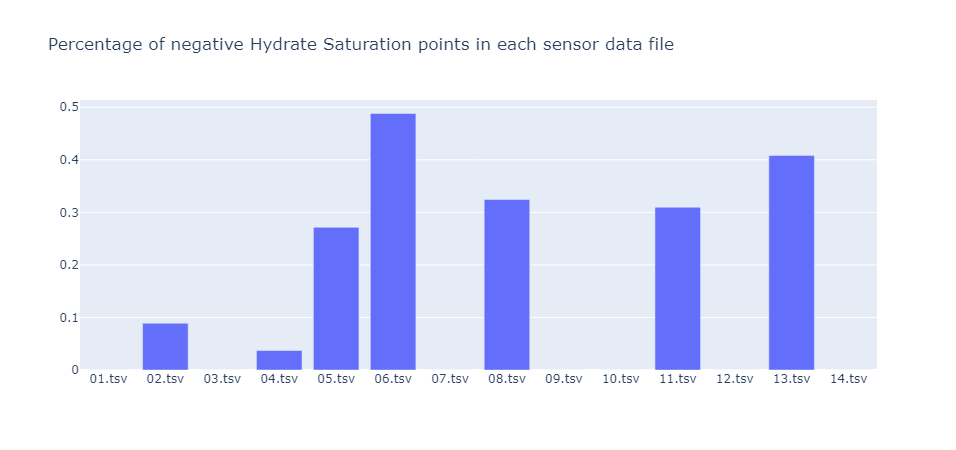
\includegraphics[width=0.5\textwidth]{figures/eda/1.png}
          \caption{含水饱和度在数据集中的负值情况}
        \end{figure}
        \begin{figure}[h]
          \centering
          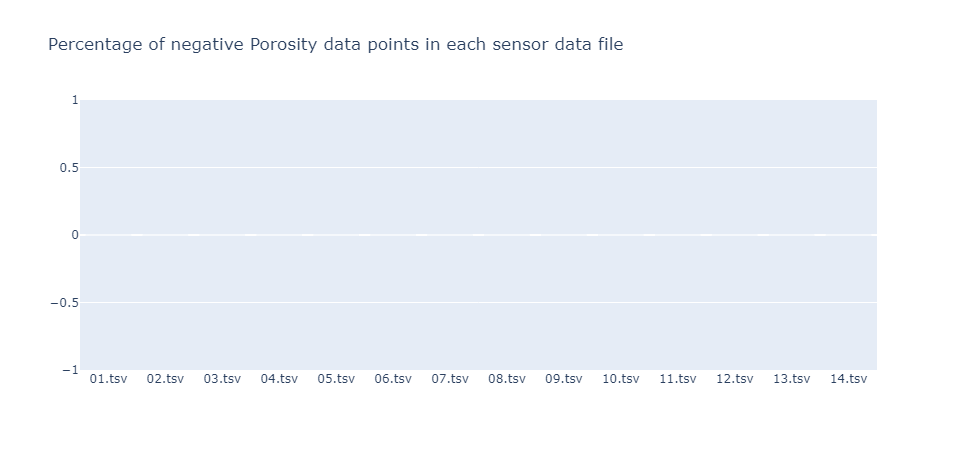
\includegraphics[width=0.5\textwidth]{figures/eda/2.png}
          \caption{孔隙度在数据集中的负值情况}
        \end{figure}
  \item \textbf{数据清洗}
        尽管常见的Min-Max标准化方法能够有效消除负值,但同时也导致了数据的失真。标准化后的数据丧失了原有的地质学意义,放弃采用。
        因此最后对原始数据集中出现的负数值全部进行了识别和剔除。
\end{enumerate}


\subsection{问题1的分析和求解}
\subsubsection{问题1模型的建立}
我们需要解决的问题是根据附件中勘探井位信息,
确定天然气水合物资源分布范围,并给出详细数据和图表,在后续分析更具体的分布奠定基础。
通过对附件一和附件二中数据的观察,钻井测量数据不仅包含了深度,还包含了孔隙度和含水合物饱和度。
天然气水合物的储层参数主要包括水合物的饱和度、分布深度、分布面积、孔隙度、渗透率等,而资源量的评估更是受到了水合物饱和度、分布深度、分布面积和孔隙度的影响。
基于成藏思路的方法从本质上来讲是体积法,
体积法能反映资源的实际状态,便于指导实际开发选址,因此是体积法最常用的水合物资源量估计方法。
其数学表达如下:
\begin{equation}
  Q = A \times Z \times \phi \times S \times E
\end{equation}
其中,$Q$ 为天然气水合物资源量,$A$ 为面积,$Z$ 为有效厚度,$\phi$ 为孔隙度,$S$ 为水合物饱和度,$E$ 为产气量因子。


\subsubsection{问题2模型的求解}
将预处理数据带入上述资源量与储层参数的线性关系,计算出天然气水合物资源量Q,通过可视化处理得到天然气水合物资源的三维深度和资源量总分布图,以及各井口内部天然气水合物资源深度与资源量的对应关系。

%????

\begin{figure}[h]
  \centering
  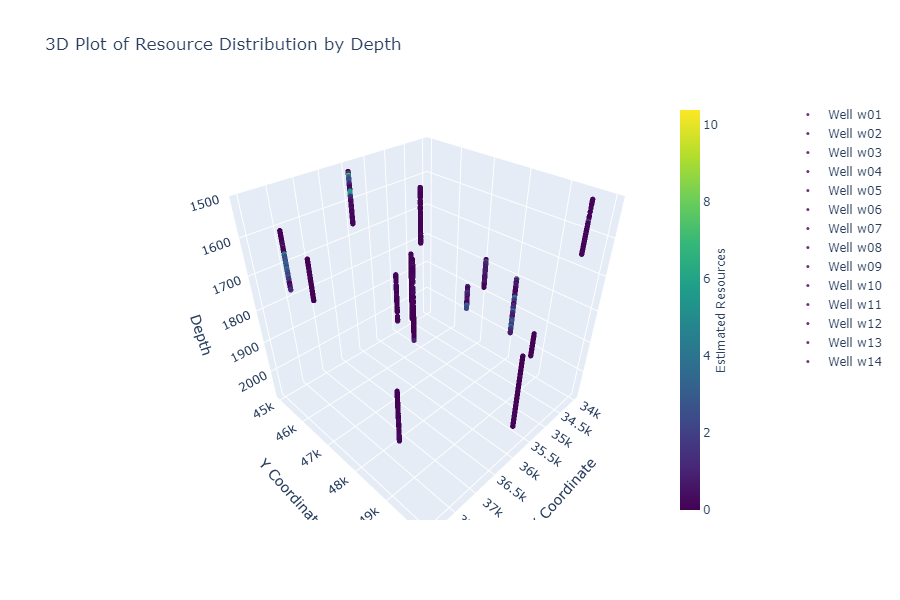
\includegraphics[width=0.5\textwidth]{figures/task1/task1-1.png}
  \caption{天然气水合物资源的三维深度和资源量总分布}
  \label{fig:3PRDD}
\end{figure}

\begin{figure}[h!t]
  \centerline{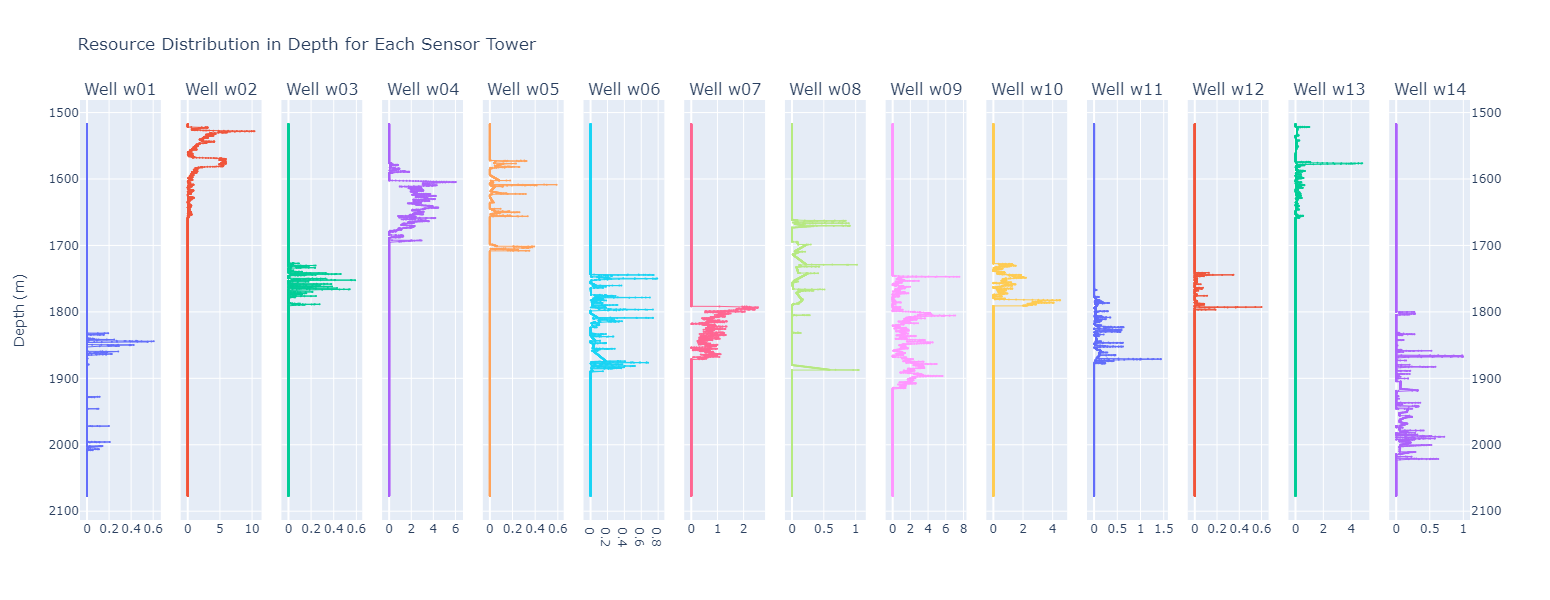
\includegraphics[scale=1]{figures/task1/task1-2.png}}
  \caption{\song\wuhao 各井口内资源深度与资源量对应关系}
\end{figure}

\begin{figure}[h!t]
  \centerline{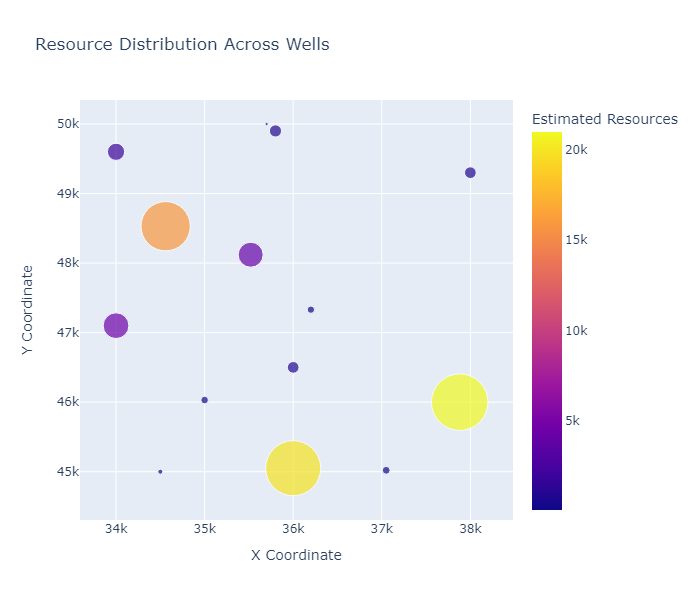
\includegraphics[scale=1]{figures/task1/task1-3.png}}
  \caption{\song\wuhao 井间资源分配}
\end{figure}


\subsubsection{问题2结果}


\subsection{问题2模型的建立和求解}
针对问题2的模型,我们首先对三个不同指标的数据进行了预处理。对于有效厚度,我们逐一分析了14口井的数据,并剔除了不需要的点,得到每口井的有效厚度列表。随后,我们将这些数据整合,并利用正态概率分布进行拟合,得到了相应的模型。对于地层孔隙度和饱和度,我们同样采用了正态概率分布进行拟合,并获得了拟合后的图像。
进一步地,我们利用14口井的所有数据,结合井的XY坐标和深度H构建了一个三维立体数据。在剔除了无用的点后,我们应用了三维Kriging插值模型进行随机拟合,得到了相应的立体图像。这一方法有助于我们理解勘探区域的变化规律,并为进一步的研究提供了重要参考。

\subsubsection{Gaussian Mixture Model}
高斯混合模型(Gaussian Mixture Model,GMM)是一种用于建模概率分布的统计模型。它由多个高斯分布组成,每个高斯分布代表了数据中的一个聚类。换句话说,GMM 假设数据是由多个高斯分布组成的混合物生成的,每个高斯分布对应于数据中的一个聚类或者一个潜在的生成过程。
GMM 是一种非监督学习算法,通常用于聚类分析,即将数据集划分为具有相似特征的子集。它也可以用于密度估计和异常检测。
在 GMM 中,每个高斯分布由其均值、协方差矩阵和权重参数表示。模型的目标是通过最大化似然函数或通过 EM 算法来估计这些参数,从而找到最佳的混合组合来解释数据。

\begin{enumerate}

  \item \textbf{GMM-参数} \\
        假设我们有一个观测数据集 $X = \{x_1, x_2, \ldots, x_N\}$,其中每个 $x_i$ 是一个 $D$ 维向量。
        \begin{itemize}
          \item \textbf{均值(mean):} $\boldsymbol{\mu_k}$,表示第 $k$ 个高斯分布的均值向量,$k = 1, 2, \ldots, K$。
          \item \textbf{协方差矩阵(covariance):} $\boldsymbol{\Sigma_k}$,表示第 $k$ 个高斯分布的协方差矩阵,$k = 1, 2, \ldots, K$。
          \item \textbf{混合系数(mixture coefficient):} $\boldsymbol{\pi_k}$,表示第 $k$ 个高斯分布在整个混合模型中的权重,$\sum_{k=1}^K \pi_k = 1$。
        \end{itemize}

  \item \textbf{GMM-Likelihood函数} \\
        \begin{equation*}
          p(X | \theta) = \prod_{i=1}^N \left( \sum_{k=1}^K \pi_k \mathcal{N}(x_i | \mu_k, \Sigma_k) \right)
        \end{equation*}
        其中 \( \mathcal{N}(x | \mu, \Sigma) \) 是多维高斯分布的概率密度函数。

  \item \textbf{GMM-模型参数估计} \\
        E 步:计算每个数据点属于每个高斯分布的后验概率
        \begin{equation*}
          \gamma(z_{ik}) = \frac{\pi_k \mathcal{N}(x_i | \mu_k, \Sigma_k)}{\sum_{j=1}^K \pi_j \mathcal{N}(x_i | \mu_j, \Sigma_j)}
        \end{equation*}

        M 步:使用后验概率重新估计参数
        \begin{align*}
          \pi_k    & = \frac{1}{N} \sum_{i=1}^N \gamma(z_{ik})                                                      \\
          \mu_k    & = \frac{\sum_{i=1}^N \gamma(z_{ik}) x_i}{\sum_{i=1}^N \gamma(z_{ik})}                          \\
          \Sigma_k & = \frac{\sum_{i=1}^N \gamma(z_{ik}) (x_i - \mu_k)(x_i - \mu_k)^T}{\sum_{i=1}^N \gamma(z_{ik})}
        \end{align*}
        重复以上 E 步和 M 步直到收敛,即参数不再变化或者变化很小。
\end{enumerate}

\subsubsection{基于GMM进行有效厚度和含水饱和度的概率分布拟合}
\begin{enumerate}
  \item \textbf{有效厚度的数据准备和预处理} \\
        我们从已有的井的数据中提取数据,采用遍历的方式,设置起始遇到可燃冰点,和终止遇到可燃冰点,得到一口井中有多少段有可燃冰的区段,然后同样的方式对其他的井进行操作,合并所有得到的段。这些段就是所有井的有效厚度列表,这个列表将用于高斯分布拟合模型的建立。

  \item \textbf{有效厚度拟合曲线} \\
        \begin{figure}[h]
          \centering
          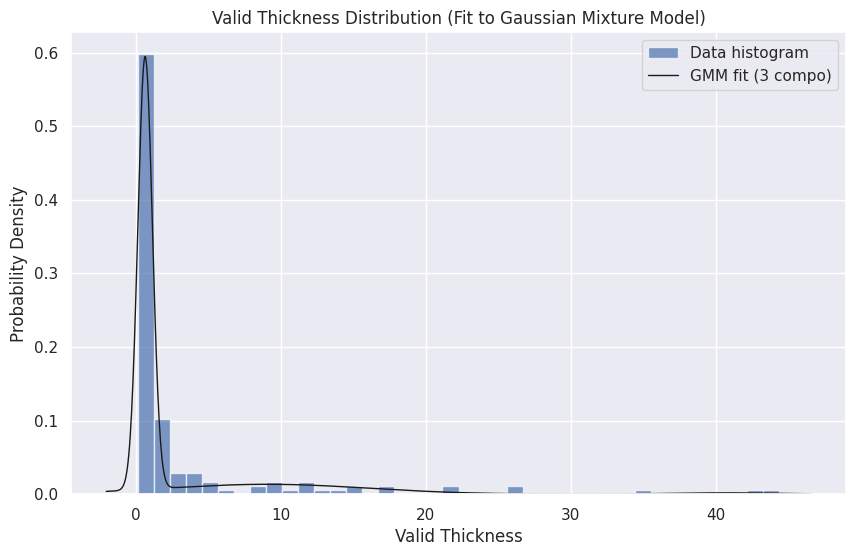
\includegraphics[width=0.8\textwidth]{figures/task2/task2-1.png}
          \caption{有效厚度的高斯混合模型}
          \label{fig:NewWellsAndResource}
        \end{figure}

        在这种情况下,通过调试参数,我们发现选择 3 个高斯分布来拟合数据效果最好,即模型在三个成分时达到了最佳的拟合效果,或者说能够最好地解释数据的分布特征。这通常表明有效厚度数据中存在三个明显的聚类或者生成机制。
  \item \textbf{含水饱和度的数据准备和预处理} \\
        将14口井的饱和度的数据放到一个tsv文件中,同时对与无效的数据以及0点进行剔除,得到一个干净的数据集,用于高斯混合模型的拟合。

  \item \textbf{含水饱和度的拟合曲线} \\
        \begin{figure}[h]
          \centering
          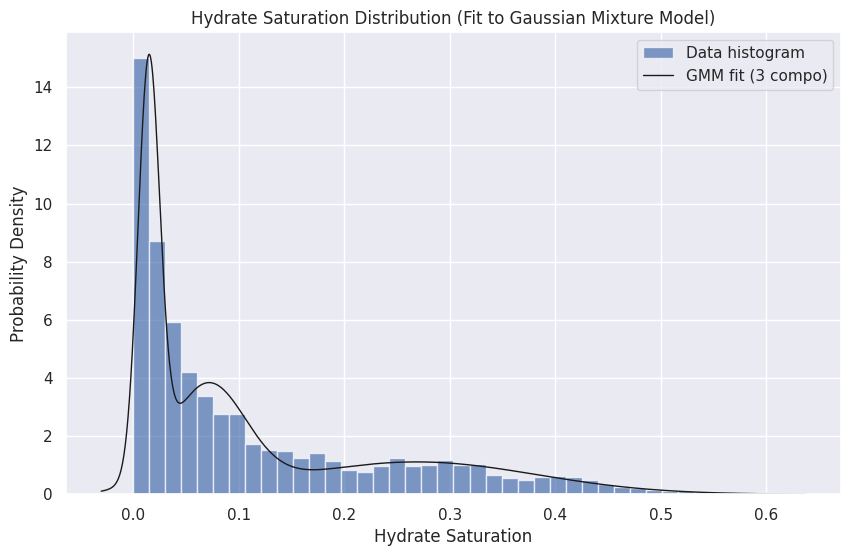
\includegraphics[width=0.8\textwidth]{figures/task2/task2-3.png}
          \caption{含水饱和度的高斯混合模型}
        \end{figure}

        在这种情况下,我们对参数进行调试,发现同样以3个高斯分布来拟合数据效果最佳,达到了理想的拟合状态。


\end{enumerate}

\subsubsection{正态分布拟合}
正态分布拟合是指使用正态分布模型来拟合观测数据的过程。在统计学和机器学习中,我们经常需要对观测数据进行建模和分析,而正态分布是一种常用的分布模型,适用于很多自然现象和实验数据。
\begin{enumerate}
  \item \textbf{正态分布定义} \\
        假设我们有一个观测数据集 $X = \{x_1, x_2, \ldots, x_N\}$,我们希望用正态分布拟合这个数据集,求出其均值 $\mu$ 和方差 $\sigma^2$。
  \item \textbf{似然函数} \\
        正态分布的概率密度函数为:
        \[
          f(x | \mu, \sigma^2) = \frac{1}{\sqrt{2\pi\sigma^2}} \exp\left(-\frac{(x - \mu)^2}{2\sigma^2}\right)
        \]
        因此,数据集的似然函数为:
        \[
          L(\mu, \sigma^2 | X) = \prod_{i=1}^N f(x_i | \mu, \sigma^2)
        \]
        取对数似然函数:
        \[
          \log L(\mu, \sigma^2 | X) = \sum_{i=1}^N \log f(x_i | \mu, \sigma^2)
        \]
  \item \textbf{最大化似然函数} \\
        我们的目标是最大化对数似然函数以估计模型参数 $\mu$ 和 $\sigma^2$。这通常通过对参数求导并令导数为零来实现。

        \subsubsection*{对 $\mu$ 求导}

        \[
          \frac{\partial}{\partial \mu} \log L(\mu, \sigma^2 | X) = \sum_{i=1}^N \frac{\partial}{\partial \mu} \log f(x_i | \mu, \sigma^2)
        \]

        利用正态分布的导数性质,我们有:
        \[
          \frac{\partial}{\partial \mu} \log f(x | \mu, \sigma^2) = \frac{x - \mu}{\sigma^2}
        \]

        代入上式,并令导数为零:
        \[
          \sum_{i=1}^N \frac{x_i - \mu}{\sigma^2} = 0
        \]

        解得:
        \[
          \mu = \frac{1}{N} \sum_{i=1}^N x_i
        \]

        这是均值 $\mu$ 的最大似然估计。

        \subsubsection*{对 $\sigma^2$ 求导}

        \[
          \frac{\partial}{\partial \sigma^2} \log L(\mu, \sigma^2 | X) = \sum_{i=1}^N \frac{\partial}{\partial \sigma^2} \log f(x_i | \mu, \sigma^2)
        \]

        利用正态分布的导数性质,我们有:
        \[
          \frac{\partial}{\partial \sigma^2} \log f(x | \mu, \sigma^2) = -\frac{1}{2\sigma^2} + \frac{(x - \mu)^2}{2\sigma^4}
        \]

        代入上式,并令导数为零:
        \[
          \sum_{i=1}^N \left( -\frac{1}{2\sigma^2} + \frac{(x_i - \mu)^2}{2\sigma^4} \right) = 0
        \]

        解得:
        \[
          \sigma^2 = \frac{1}{N} \sum_{i=1}^N (x_i - \mu)^2
        \]

        这是方差 $\sigma^2$ 的最大似然估计。
\end{enumerate}

\subsubsection{基于正态分布进行孔隙度的概率分布拟合}
\begin{enumerate}
  \item \textbf{孔隙度的数据准备和预处理} \\
        将14口井的地层孔隙度的数据放到一个tsv文件中,同时对与无效的数据以及0点进行剔除,得到一个干净的数据集,用于正态模型的拟合。

  \item \textbf{孔隙度拟合曲线} \\
        \begin{figure}[h]
          \centering
          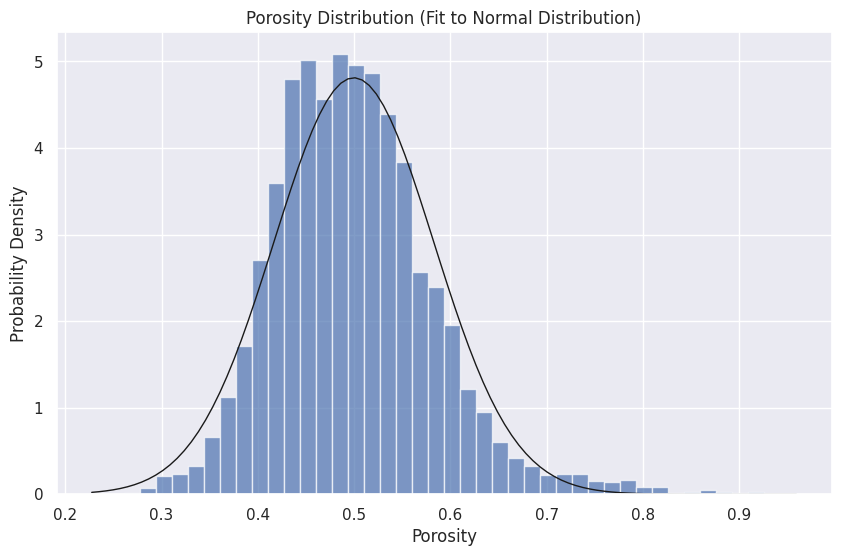
\includegraphics[scale=0.5]{figures/task2/task2-2.png}
          \caption{孔隙度的正态分布模型}
        \end{figure}

        在这种情况下,通过调试参数,我们发现正态分布的拟合效果最佳,达到了预期的效果。

\end{enumerate}

\subsubsection{Kernel Density Estimation}
核密度估计(Kernel Density Estimation,KDE)是一种非参数方法,用于估计连续随机变量的概率密度函数。它通过在每个观测数据点周围放置核函数(通常是高斯核函数),然后对所有核函数进行加权平均来估计密度。

KDE 的基本公式为:
\[
  \hat{f}_h(x) = \frac{1}{n} \sum_{i=1}^{n} K_h(x - x_i)
\]
其中:
\begin{itemize}
  \item \( \hat{f}_h(x) \) 是在点 \( x \) 处估计的密度;
  \item \( n \) 是数据点的数量;
  \item \( x_i \) 是观测数据点;
  \item \( K_h(\cdot) \) 是核函数,通常是高斯核函数,参数 \( h \) 是带宽(bandwidth),用于控制核函数的宽度。
\end{itemize}

高斯核函数 \( K_h(u) \) 的形式为:
\[
  K_h(u) = \frac{1}{\sqrt{2\pi}h} \exp\left(-\frac{u^2}{2h^2}\right)
\]

KDE 的一个关键参数是带宽 \( h \),它决定了核函数的宽度。较小的带宽会导致更细致的估计,但可能会产生过拟合;较大的带宽会导致平滑的估计,但可能会丢失一些细节。因此,选择合适的带宽对于获得良好的密度估计至关重要。

KDE 在数据可视化、密度估计、异常检测等领域都有广泛的应用。它提供了一种灵活的方法来估计数据的概率密度函数,不受特定分布形式的限制。

\subsubsection{基于KDE进行有效厚度变化规律分析}

我们利用之前GMM准备好的数据采用了KDE,生成了一个二维的color mesh图。
\begin{figure}[h]
  \centering
  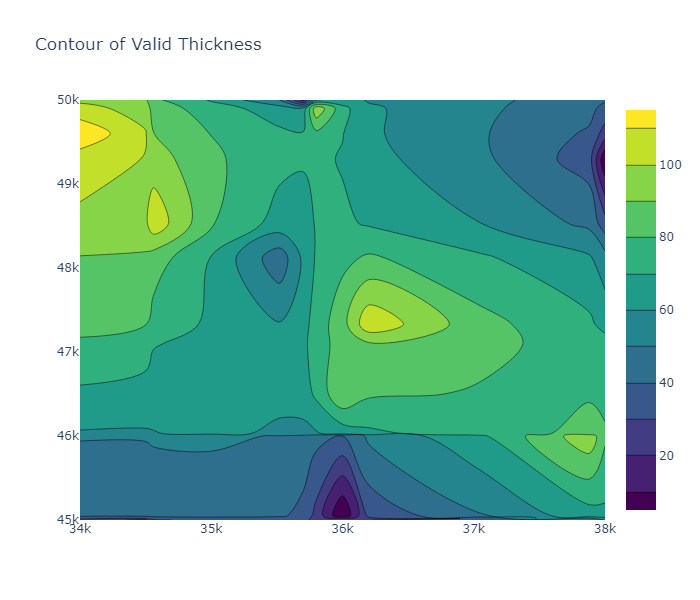
\includegraphics[width=0.8\textwidth]{figures/task2/task2-4.png}
  \caption{有效厚度的变化规律图}
  \label{fig:NewWellsAndResource}
\end{figure}

\subsubsection{空间三维的Kriging模型}
Kriging 是一种插值和空间预测技术,常用于地理空间数据分析、地质勘探、环境科学等领域。它基于空间统计学的原理,通过对已知数据点之间的空间相关性进行建模,来预测未知位置的数值。
\begin{enumerate}
  \item \textbf{基本假设} \\
        假设我们有 $n$ 个已知的观测点 $(x_i, y_i, z_i)$,对应的观测值为 $Z(x_i, y_i, z_i)$,我们希望在未知点 $(x, y, z)$ 处估计变量值 $Z(x, y, z)$。

  \item \textbf{半方差函数的定义} \\
        假设 $h$ 是空间上两个点之间的距离,我们定义半方差函数 $\gamma(h)$ 为:

        \[
          \gamma(h) = \frac{1}{2} \text{Var}[Z(x_i, y_i, z_i) - Z(x_i+h, y_i+h, z_i+h)]
        \]

        其中,$\text{Var}[\cdot]$ 表示方差。这个公式描述了在距离 $h$ 处的两个点之间变量值的变化程度。
  \item \textbf{克里金模型的基本公式} \\
        克里金模型的基本公式为:

        \[
          Z(x, y, z) = \sum_{i=1}^{n} \lambda_i \cdot Z(x_i, y_i, z_i)
        \]

        其中,$\lambda_i$ 是权重,用于对已知点的观测值进行加权求和。
  \item \textbf{最小均方误差} \\
        我们希望通过最小化预测值 $Z(x, y, z)$ 与真实值 $Z(x, y, z)$ 之间的均方误差来确定权重 $\lambda_i$。
  \item \textbf{最小化均方误差的优化问题} \\
        定义误差 $e(x, y, z) = Z(x, y, z) - \sum_{i=1}^{n} \lambda_i \cdot Z(x_i, y_i, z_i)$,则我们的目标是最小化误差的平方和:

        \[
          \min_{\lambda_i} \sum_{i=1}^{n} e^2(x, y, z)
        \]

\end{enumerate}


\subsubsection{基于Kriging进行孔隙度和含水饱和度的变化规律分析}
\begin{enumerate}
  \item \textbf{孔隙度在空间中的数值分布} \\
        \begin{figure}[h]
          \centering
          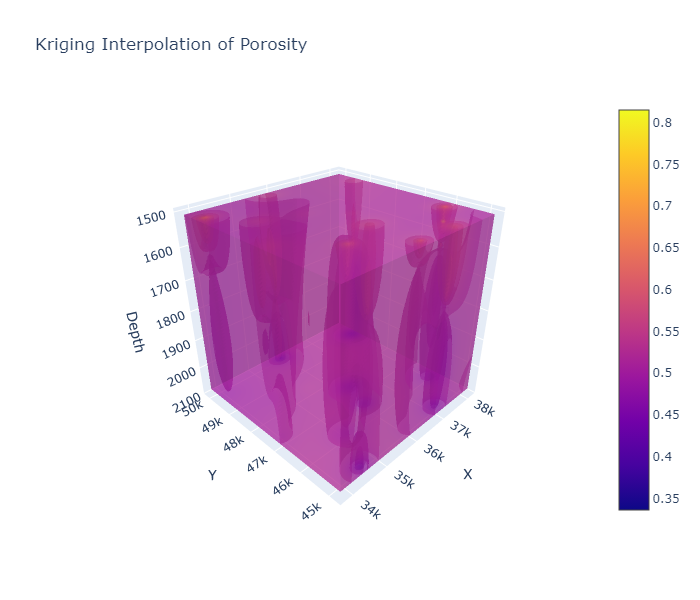
\includegraphics[scale=0.4]{figures/task2/task2-5-1.png}
          \caption{孔隙度Kriging3D图}
          \label{fig:porosity-Kriging-3d}
        \end{figure}
  \item \textbf{孔隙度在空间中的数值分布误差} \\
        \begin{figure}[h]
          \centering
          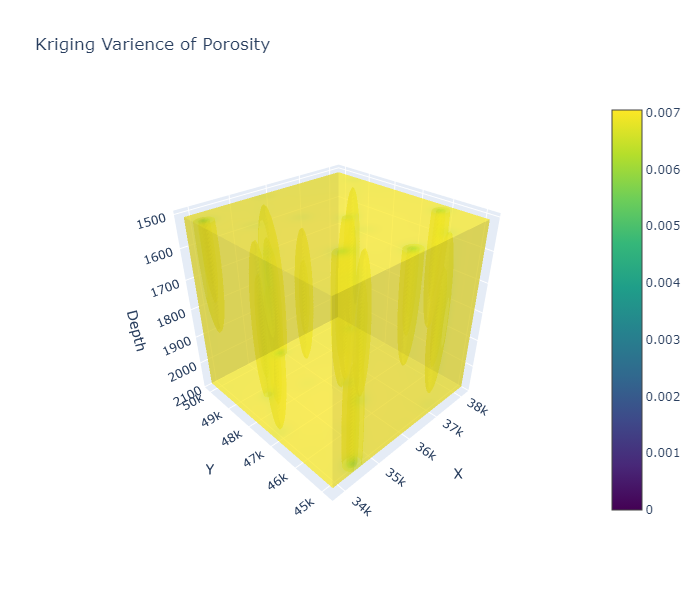
\includegraphics[scale=0.4]{figures/task2/task2-5-2.png}
          \caption{孔隙度Kriging3D误差图}
          \label{fig:porosity-error-Kriging-3d}
        \end{figure}

  \item \textbf{含水饱和度在空间中的数值分布} \\
        \begin{figure}[h]
          \centering
          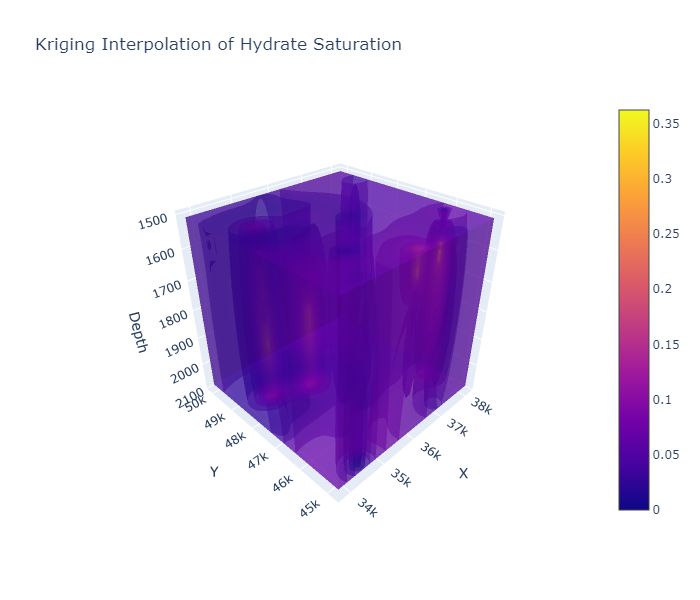
\includegraphics[scale=0.4]{figures/task2/task2-6-1.png}
          \caption{含水饱和度Kriging3D图}
          \label{fig:water-saturation-Kriging-3d}
        \end{figure}
  \item \textbf{含水饱和度在空间中的数值分布误差} \\
        \begin{figure}[h]
          \centering
          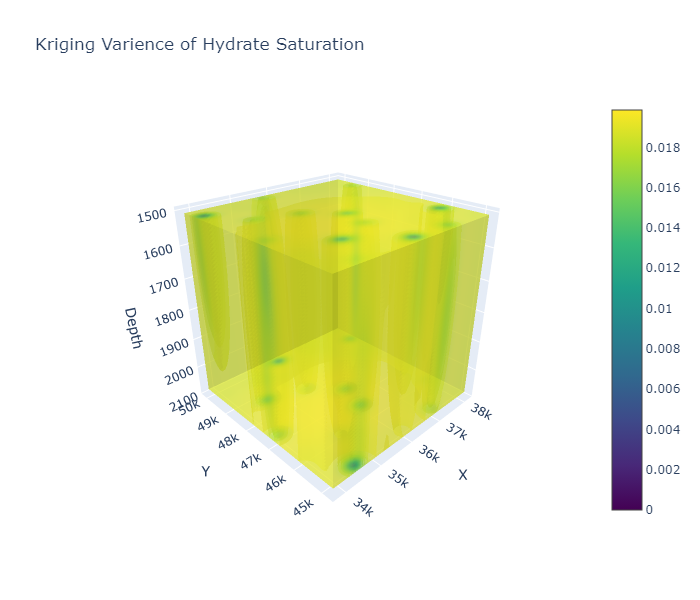
\includegraphics[scale=0.4]{figures/task2/task2-6-2.png}
          \caption{含水饱和度Kriging3D误差图}
          \label{fig:water-saturation-error-Kriging-3d}
        \end{figure}

\end{enumerate}



\subsection{问题3模型的建立和求解}

\subsubsection{问题3模型的建立}
对于资源量的概率分布估计,我们沿用了问题2中的二维 KDE 方法,通过核密度估计来估计资源量的概率分布,并且依然采用高斯内核。

因此 KDE 计算表达式为:
\[
  f(x, y) = \frac{1}{Q_k} \sum_{i=1}^{Q_k} \frac{1}{2\pi h^2} \exp \left( -\frac{(x-x_i)^2 + (y-y_i)^2}{2h^2} \right)
\]

而对于勘探区域内资源总量的估计,我们可以直接利用问题2中得到的孔隙度和饱和度的 Kringing 插值结果,估算空间内每个位置点的资源量,所有求和即可得到总资源量的概率分布估计。

对于这个建模我们可以得到表达式:
\[
  Q_k =
\]
\[
  Q_{\text{total}} = \sum_{k=1}^{n} Q_k
\]

\subsection{问题4模型的建立和求解}
\subsubsection{二维 Kriging 插值模型的建立}
二维 Kriging 插值是一种高级的地统计学方法,用于预测空间数据的分布。在本研究中,我们使用普通Kriging模型(Ordinary Kriging)来估计未知位置的资源量,基于已知井点的资源数据。

\begin{enumerate}
  \item \textbf{数据准备和预处理} \\
        首先,我们从已有的井点数据中提取坐标 $(x_i, y_i)$ 和对应的资源量 $z_i$。这些数据点作为Kriging插值的输入,用于构建空间连续性模型。

  \item \textbf{普通Kriging模型} \\
        普通Kriging模型的基本公式可以表示为:
        \[
          Z(x) = \mu + \sum_{i=1}^n \lambda_i (Z(x_i) - \mu)
        \]
        其中,$Z(x)$ 是在位置 $x$ 的预测值,$\mu$ 是未知常数(通常是全局均值),$Z(x_i)$ 是已知数据点的值,$\lambda_i$ 是权重系数,$n$ 是用于预测的已知数据点的数量。

  \item \textbf{变异函数和模型参数} \\
        在Kriging方法中,变异函数(semivariogram)是描述空间数据点之间关系的关键。在本研究中,我们选择球形变异函数模型,其表达式为:
        \[
          \gamma(h) =
          \begin{cases}
            C_0 + C \left( \frac{3h}{2a} - \frac{h^3}{2a^3} \right) & \text{if } h \leq a \\
            C_0 + C                                                 & \text{if } h > a
          \end{cases}
        \]
        其中,$h$ 是空间距离,$C_0$ 是块金效应(nugget effect),$C$ 是基台值(sill),$a$ 是变程(range),即空间相关性的最大距离。

  \item \textbf{权重系数的确定} \\
        权重系数 $\lambda_i$ 通过解决Kriging方程来确定,确保预测误差最小化。Kriging方程可以表示为:
        \[
          \sum_{j=1}^n \lambda_j \gamma(x_i, x_j) + \mu = \gamma(x_i, x)
        \]
        对于所有 $i = 1, 2, \ldots, n$。此外,为了保证无偏估计,权重的和应该满足:
        \[
          \sum_{i=1}^n \lambda_i = 1
        \]

  \item \textbf{插值和预测} \\
        最后,使用解得的权重系数 $\lambda_i$ 和模型参数,我们可以计算任意位置 $x$ 的资源量预测值 $Z(x)$。这一过程涉及到在整个研究区域内创建一个平面网格,并在每个网格点上应用上述Kriging公式进行资源量预测。
\end{enumerate}

\subsubsection{二维 Kriging 插值模型的求解}

\begin{enumerate}
  \item \textbf{实验半方差图结果分析} \\
        % Insert pics
        \begin{figure}[h]
          \centering
          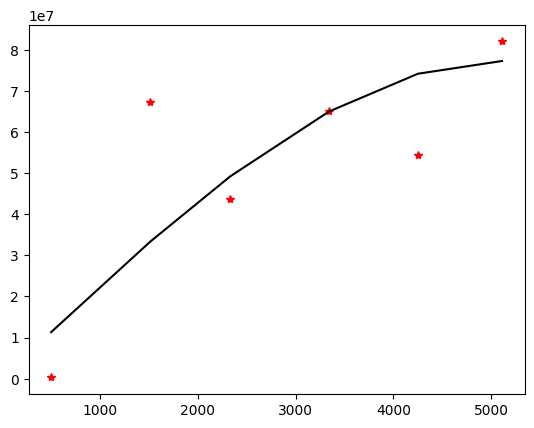
\includegraphics[width=0.4\textwidth]{figures/task4/task4-1.png}
          \caption{实验半方差图结果}
          \label{fig:KrigingSemivariogram}
        \end{figure}
        如图 \ref{fig:KrigingSemivariogram} 所示,实验半方差图显示了理论模型(黑色曲线)与实际观测数据点(红色星号)的对比。主要观察结果包括:
        \begin{itemize}
          \item 实际数据点大体上遵循理论模型的趋势,表明所选的球形变异函数模型是合适的。
          \item 在较小的空间距离 \( h \) 上,数据点与理论曲线较为接近,说明在小范围内,空间自相关性较强。
          \item 随着 \( h \) 的增加,实际数据点的分布开始波动,可能反映了在较大距离上空间自相关性的减弱。
        \end{itemize}

  \item \textbf{预测误方差与插值结果分析} \\
        \begin{figure}[h]
          \centering
          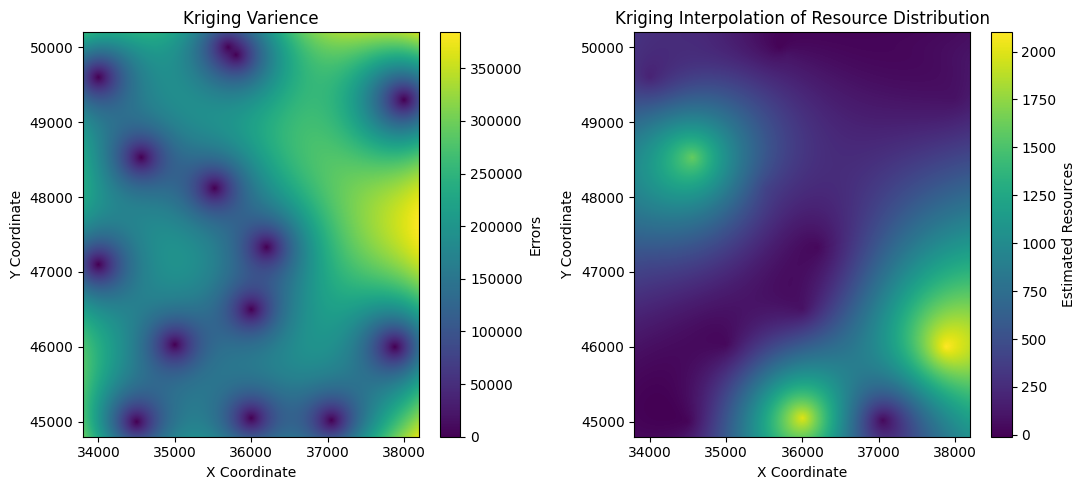
\includegraphics[width=0.8\textwidth]{figures/task4/task4-2.png}
          \caption{预测误方差(左)和 插值结果(右)}
          \label{fig:KrigingInterpolation}
        \end{figure}
        第二张图片(图 \ref{fig:KrigingInterpolation})展示了 Kriging 预测的方差(左图)和资源量的插值结果(右图)。分析如下:
        \begin{itemize}
          \item \textbf{预测误方差图(左图)}:
                \begin{itemize}
                  \item 显示了各个位置的预测误差大小,颜色越亮(趋向黄色)表示预测的不确定性越大。
                  \item 在已知数据点附近,预测误差较小,显示模型在数据点附近具有较高的信度。
                  \item 数据点间的区域预测误差增大,反映了这些区域内插值的不确定性较高。
                \end{itemize}
          \item \textbf{资源量插值结果图(右图)}:
                \begin{itemize}
                  \item 此图显示了整个区域的资源量预测分布。颜色越亮(趋向黄色)表示预测的资源量越高。
                  \item 资源量的高值区主要集中在某些特定区域,可能与原始数据点的分布和地质特性有关。
                  \item 插值结果显示了资源分布的空间变异性,有助于理解资源在研究区域内的分布特征。
                \end{itemize}
        \end{itemize}

        我们还利用二维 Kriging 插值的结果再次估计勘探区域的资源总量,即
        \[
          Q_{\text{total}} = \sum_{k=1}^{n} Q_k
        \]。
        最终的到 50355145428.42452 的结果,这与问题三中利用孔隙度和饱和度三维 Kringing 插值结果求出的资源总量 44417499906.32 误差仅约为 10\%,间接验证了模型的准确性。

\end{enumerate}



\subsubsection{粒子群优化算法的数学模型}
粒子群优化(PSO)是一种基于群体的优化技术,模拟鸟群的社会行为来寻找问题的最优解。每个粒子代表潜在的解决方案,在解空间中按照简单的数学规则移动。

\begin{enumerate}
  \item \textbf{粒子的表示} \\
        在PSO中,粒子$i$在$d$维搜索空间中的位置表示为$\mathbf{x}_i = (x_{i1}, x_{i2}, \ldots, x_{id})$,速度表示为$\mathbf{v}_i = (v_{i1}, v_{i2}, \ldots, v_{id})$。每个粒子还维护一个个人最优位置$\mathbf{p}_{\text{best},i}$,即该粒子历史上遇到的最优位置。

  \item \textbf{速度和位置更新} \\
        粒子的速度和位置通过以下公式更新:
        \[
          \mathbf{v}_i^{(t+1)} = w \mathbf{v}_i^{(t)} + c_1 r_1 (\mathbf{p}_{\text{best},i} - \mathbf{x}_i^{(t)}) + c_2 r_2 (\mathbf{g}_{\text{best}} - \mathbf{x}_i^{(t)})
        \]
        \[
          \mathbf{x}_i^{(t+1)} = \mathbf{x}_i^{(t)} + \mathbf{v}_i^{(t+1)}
        \]
        其中,$w$是惯性权重,控制粒子速度的保留程度;$c_1$和$c_2$是学习因子,通常称为认知和社会参数;$r_1$和$r_2$是[0,1]区间内的随机数,代表随机性;$\mathbf{g}_{\text{best}}$是全局最优位置,即所有粒子历史上遇到的最优位置。

  \item \textbf{参数选择} \\
        惯性权重$w$通常设置为0.7至0.9之间,有助于控制搜索的全局和局部探索能力。学习因子$c_1$和$c_2$通常设置为相同的值,比如1.5,这样可以平衡个体经验和群体经验的影响。

  \item \textbf{初始化和迭代过程} \\
        每个粒子的初始位置和速度通常是随机生成的。在每次迭代中,根据上述规则更新所有粒子的速度和位置。同时,更新每个粒子的个人最优位置以及全局最优位置。迭代继续进行,直到满足最大迭代次数或其他终止条件。

  \item \textbf{目标函数和优化目标} \\
        PSO目标是找到使目标函数$J(x)$最大化的解$\mathbf{x}$。在本文中,目标函数是最大化新井位置的预测资源总量和最小化井点间的最短距离的负值。
\end{enumerate}


\subsubsection{基于 Kriging 插值的优化模型建立}

在 Kriging 模型的求解结果和粒子群优化算法的基础上,我们进一步建立了一个优化模型,旨在确定新井的最佳位置,以最大化资源的总探测量和井点之间的距离。模型的目标函数综合考虑了新井之间以及新旧井之间的最小距离和新井位置的预测资源总量。

\begin{enumerate}
  \item \textbf{目标函数定义} \\
        设计目标函数如下,用于评估新井布置的质量:
        \[
          J(x) = -\left(\min(\text{dist}(x_i, x_j)) + \sum_{k=1}^{n} Z(x_k, y_k)\right)
        \]
        其中,$n$ 为新井的数量,$x = \{(x_1, y_1), (x_2, y_2), \ldots, (x_{n}, y_{n})\}$ 表示新井的位置,$\text{dist}(x_i, x_j)$ 表示所有井点(包括现有和新井)之间的欧氏距离矩阵,$Z(x_k, y_k)$ 是在位置 $(x_k, y_k)$ 的预测资源量,通过 Kriging 插值得到。

  \item \textbf{优化算法选择} \\
        我们采用粒子群优化(PSO)算法来解决这一多目标优化问题。PSO 是一种基于群体的随机优化技术,通过模拟鸟群的社会行为来搜索最优解。在本问题中,每个粒子代表一组潜在的新井位置,粒子通过迭代更新其位置,以寻找使目标函数最大化的解。

  \item \textbf{粒子群优化参数设置} \\
        在 PSO 算法中,我们设置了如下参数:个体学习因子$c_1$、社会学习因子$c_2$和惯性权重$w$。这些参数控制粒子更新其速度和位置的方式,其中$c_1$和$c_2$通常设置为1.5,$w$设置为0.7。

  \item \textbf{约束条件和边界} \\
        新井的位置受到现有井位置的范围约束,即每个新井的坐标$(x, y)$必须在现有井的最小和最大坐标加上了 150 m 扩展的范围内。这确保了新井的位置在合理的探测区域内。

  \item \textbf{优化执行} \\
        优化过程包括初始化一定数量的粒子,每个粒子代表一组新井的位置。通过迭代,每个粒子根据其自身经验和群体经验更新位置,直到达到最大迭代次数或满足其他终止条件。最终,算法输出最优的新井位置和相应的目标函数值。
\end{enumerate}

\subsubsection{优化模型的求解}
在本节中,我们将详细分析基于Kriging插值和粒子群优化算法(PSO)建立的优化模型的求解结果。该模型的目标是确定新井的最佳位置,以最大化资源的探测量并优化井点之间的距离。
\begin{enumerate}

  \item \textbf{新井位置优化结果}

        \begin{figure}[h]
          \centering
          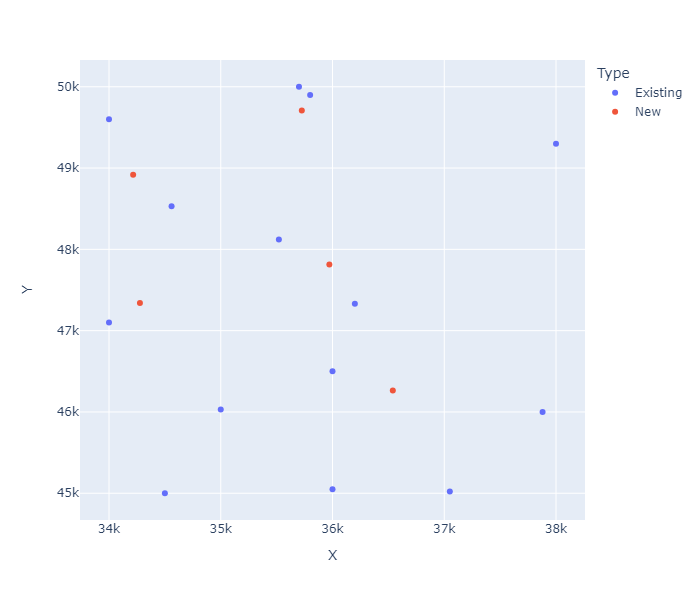
\includegraphics[width=0.5\textwidth]{figures/task4/task4-3.png}
          \caption{新井位置优化结果}
          \label{fig:NewWellsAndOldWells}
        \end{figure}
        首先,我们从新井的布局开始。如图 \ref{fig:NewWellsAndOldWells} 所示,新井(红色点)与现有井(蓝色点)的布局展示了新井的选址策略不仅考虑了资源量的最大化,同时也确保了合理的空间分布,避免过于集中或偏远。


  \item \textbf{资源量和不确定性分析}

        \begin{figure}[h]
          \centering
          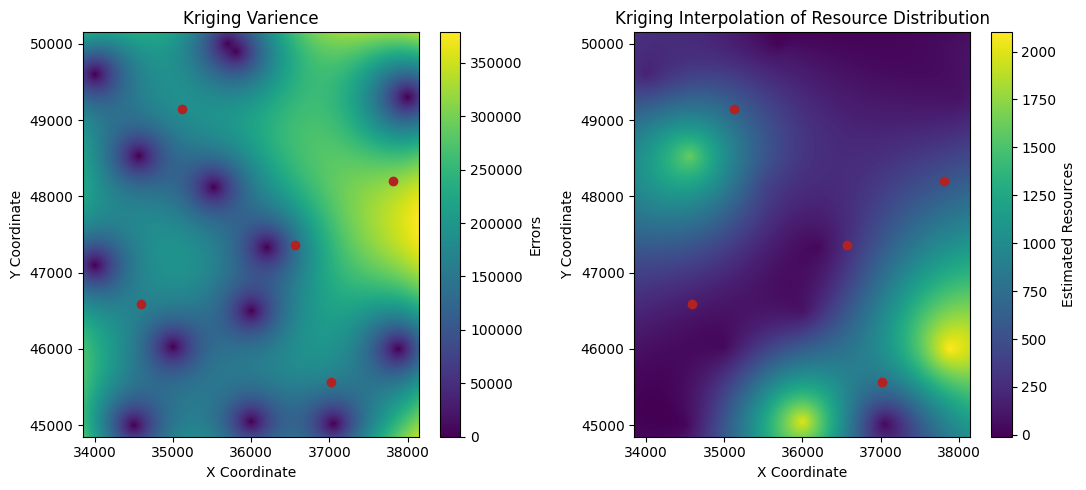
\includegraphics[width=0.8\textwidth]{figures/task4/task4-4.png}
          \caption{新井位置资源量情况}
          \label{fig:NewWellsAndResource}
        \end{figure}
        接下来,我们通过Kriging插值的结果来分析资源量分布和不确定性。如图 \ref{fig:NewWellsAndResource} 右侧所示,Kriging插值的资源分布图显示了预测的资源量,其中颜色越暗表示资源量越高。这帮助我们验证新井位置的选择是否位于资源丰富的区域。左侧的Kriging方差图表则提供了关于预测不确定性的信息,颜色越亮表示不确定性越高,这通常出现在样本点较少的区域。


  \item \textbf{井点距离的离散程度分析}
        \begin{figure}[h]
          \centering
          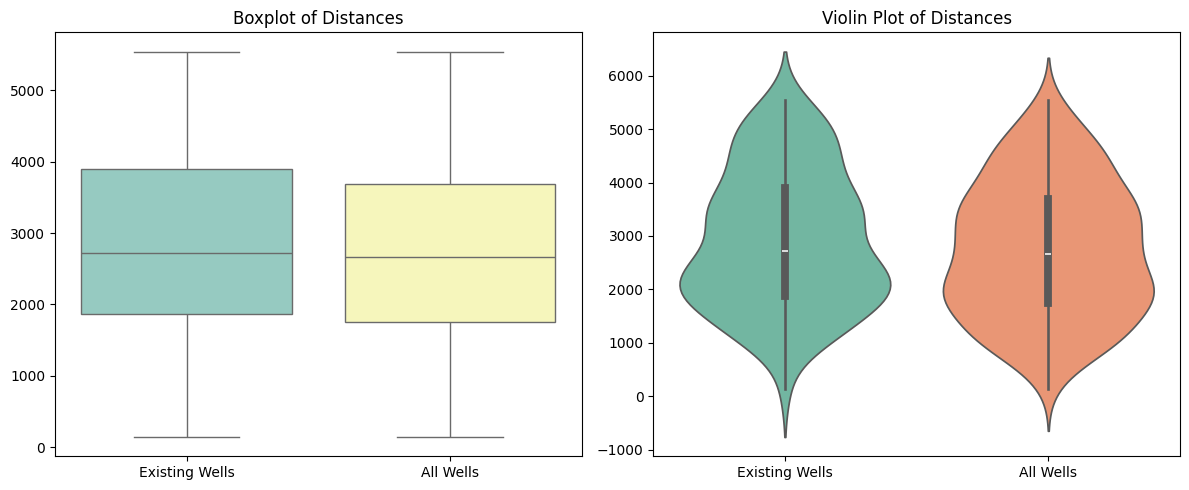
\includegraphics[width=0.8\textwidth]{figures/task4/task4-5.png}
          \caption{添加新井前后,所有井距离的离散程度}
          \label{fig:NewWellsAndNoNewWells}
        \end{figure}

        最后,我们分析了添加新井前后所有井点距离的离散程度。如图 \ref{fig:NewWellsAndNoNewWells} 所示,通过箱型图和小提琴图可以看出,引入新井后,井点之间的距离的中位数有所降低,这表明新井的加入使得井点分布更加均匀。小提琴图进一步揭示了数据分布的密度和范围,展示了新井引入前后井点距离分布的变化。

\end{enumerate}


\section{模型的评价与推广 模型的评价与推广}

\textcolor{red}{将模型进行数值计算,并与附件中的真实采样值(进行列表或图示)比较。对误差进行数据分析,给出误差分析的理论估计。}


\subsection{模型的评价}
\subsubsection{模型的优点}
\textcolor{red}{得到满意的解、
  较好地解决了$\cdots$问题、
  使模型得到简化、
  使结果更合理,避免…带来的较大误差、
  使问题描述比较清晰、
  减少大的计算量。
}
\begin{enumerate}
  \item 模型假设与现实差异:本研究中所建立的模型基于一系列关键假设,包括对地壳稳定性和参数均一性的考虑,但现实世界的地质情况远比模型所能涵盖的要复杂得多。模型仅仅在特定条件下的理论上是健全的,但可能无法始终准确预测所有现实世界条件下的地质现象。
  \item 模型参数的局限性:
        鉴于题目所提供的条件和指导,我们的模型在构建时未能纳入所有可能影响结果的参数。模型中的参数没有进行全面的自相关和共线性分析,这可能会影响到模型的预测能力。未来的研究可以引入更广泛的参数集和更详细的分析。
  \item 误差与数据量的讨论:
        预测精度受到了数据量不足的限制,导致了较多的误差。我们默认数据中的潜在误差不存在。数据的预处理可以更加精确(加上你们前面说的误差)
\end{enumerate}

该模型较为精准的得到了题目要求的内容,包括

(1)问题求解中 辅之流程图, 将建模思路完整清晰的展现出来;
(2)问题二在对 问题二在对理论通行能力进修复时考虑因素 细致、全面,理论通行能力进修复时考虑因素
细致、全面,系数准确度高;
(3)在问题三中,提出“影响度”的概念较为直观地定量给小区开放后的效果,简便有.在影响度计算上由
点及面从每个路段、交叉口到整 个路网,层深入具有逻辑性;
(4)运用多种数学软件(如 MATLAB、SPSS),取长补短,使计算结果更加),取长补短,使计算结果更
加 准确、明晰.

\subsubsection{模型的缺点}
\textcolor{red}{主观性过强、
  建立在什么的前提条件下、
  有一定的局限性、
  存在不确定性、
  有一定的偏差。
}
\begin{enumerate}
  \item 模型假设与现实差异:本研究中所建立的模型基于一系列关键假设,包括对地壳稳定性和参数均一性的考虑,但现实世界的地质情况远比模型所能涵盖的要复杂得多。模型仅仅在特定条件下的理论上是健全的,但可能无法始终准确预测所有现实世界条件下的地质现象。
  \item 模型参数的局限性:
        鉴于题目所提供的条件和指导,我们的模型在构建时未能纳入所有可能影响结果的参数。模型中的参数没有进行全面的自相关和共线性分析,这可能会影响到模型的预测能力。未来的研究可以引入更广泛的参数集和更详细的分析。
  \item 误差与数据量的讨论:
        预测精度受到了数据量不足的限制,导致了较多的误差。我们默认数据中的潜在误差不存在。数据的预处理可以更加精确(加上你们前面说的误差)
\end{enumerate}


\subsection{模型的推广与优化}
本文中采用的体积法模型在天然气水合物资源评估中表现出一定的效率和实用性,尤其适用于具有相对均一地质特征和充分数据支持的区域。然而,为了增强模型的广泛适用性和准确度,以下提出一些可能的推广和优化方向,这些方向虽然需要进一步研究和验证,但具有较高的创新潜力和实用价值。
\begin{enumerate}
  \item 集成动态地质过程模拟:尽管体积法提供了一个静态的资源评估框架,但真实的地质过程是动态的,包括温度、压力的变化以及相关的地质活动。可以考虑开发一种集成模型,该模型能够模拟和预测这些动态过程对天然气水合物稳定性和可开采性的影响。通过引入时间维度,模型不仅能估算当前的资源量,还能预测资源的未来可利用性。
  \item 引入空间统计和地统计学方法:为了更精确地处理地质参数的空间变异性,模型可以集成先进的空间统计和地统计学方法,如变异函数分析和多点统计模拟。这些方法可以更好地描述和模拟地质参数的空间相关性和不确定性,提高资源量估算的空间精度。
  \item 经济因素的集成分析:在资源评估模型中引入经济学参数,如开采成本、市场价格和技术进步,可以构建一个更加综合的评估模型。这种经济-地质集成模型不仅可以预测资源量,还可以提供资源开发的经济可行性分析,为决策者提供更全面的决策支持。
  \item  多尺度模型开发:开发一个多尺度模型,可以同时处理区域尺度和局部尺度的地质数据。这种模型能够综合考虑大范围的地质结构特征与小范围的地质细节,提供更为精细化的资源评估。
  \item  可持续性评估的集成:在模型中加入环境影响评估模块,可以预测资源开发对环境的潜在影响,如温室气体排放、生态干扰等。这种集成可以帮助制定更为可持续的资源开发策略,符合全球可持续发展的要求。
\end{enumerate}
为了确保模型的准确性不受损害,我们舍弃了数据集里面的大量异常点,以提高数据质量,以避免任何可能的偏差对分析结果造成不利影响。尽管这一做法无可避免地导致了信息的损失,但它是确保研究严谨性的必要步骤,我们对于无法将它们纳入最终模型表示遗憾。如果不受时间限制的约束,我们可以投入更多的时间和资源,对全部数据点进行深入分析和处理。这将使我们能够构建一个更为全面和精确的模型,从而更准确地反映数据的真实分布和内在关系。


\section{模型的改进}

\subsection{模型一的改进}
针对问题二中的模型一,在具体求解大型车对车辆通行能力的修正系数时,
我们利用交通量的测算值对照得到相应的大型车修正系数.但是,在实际操作中
交通量的测定有很大的难度,如果此时交通量数据无法得到,那么我们便不能得
到相应的修正系数,因此我们对模型进行改进.

由~GREENSHIELD K-V 线性模型,可得通行能力的公式:
\begin{align}
  A_{p}=\begin{cases}
          \dfrac{3600}{t}\left(1-\dfrac{3.6 l}{V_{t} t}\right)\left(V_{f}>7.2 l / t\right) \\
          \dfrac{250 V_{f}}{t}\left(V_{f} \leq 7.2 l / t\right)
        \end{cases}
\end{align}

对应的临界车辆速度:
\begin{align}
  V_{p}=\begin{cases}
          \dfrac{V_{f}-3.6 l}{t} & \left(V_{f}>7.2 l / t\right)      \\
          \dfrac{1}{2} V_{f}     & \left(V_{f} \leq 7.2 l / t\right)
        \end{cases}
\end{align}

由美国道路通行能力准则可得,美国将道路服务水平分为六级:A-F 级,而
我国目前针对当前国情,将道路服务水平分成四级:一级相当于美国的A、B 两
级;二级相当于美国的C 级;三级相当于美国的D 级;四级相当于美国的E、F
级。因此,相应的,将美国服务水平划分标准进行针对性修正,得到中国道路服
务水平划分标准,见表

\begin{table*}[h!]
  \centering
  \small
  \tabcolsep 2pt
  \caption{我国服务水平划分标准}
  \begin{tabular*}{0.87\linewidth}{p{60pt}<{\centering}p{40pt}<{\centering}
    p{40pt}<{\centering}p{40pt}<{\centering}p{40pt}<{\centering}
    p{80pt}<{\centering}p{40pt}<{\centering}}
    \toprule
    服务水平 (L0S)  & \multicolumn{2}{c} {一级 } & 二级  & 三级  & \multicolumn{2}{c} {四级 } \\
    \cline{2-3}\cline{6-7}
    服务交通量  & 800 & 1200 & 1800 & 2500 & $A_{D}$ & $\leqslant A_{P}$ \\
    速度  km / h & 120 & 120 & 120 & 120 & $\geqslant V_{p}$ & $\leqslant V_{p}$ \\
    V / C & 0.33 & 0.48 & 0.71 & 1.0 & $A_{p} / A_{\max}\leqslant 1.0$ & -(无意义 ) \\
    \bottomrule
  \end{tabular*}
\end{table*}

由于车流量的测算相对于交通量来说较易得到,我们便可以不用对交通量进
行测算,可以通过车流量与通行能力的比值计算出~V/C 饱和度值,再通过该值对
照我国服务水平划分标准,间接得到服务交通量,从而得到大型车对通行能力的
修正系数.


\subsection{模型二的改进}

针对于问题三中的模型,在得出各个类型小区在开放后对于整个小区周边路
网交通负荷影响度后,无法判别小区开放的效果是积极的还是消极的,由此我们
可以采用~Bress 悖论的原理进行判别:在个人独立选择路径的情况下,为某路网
增加额外的通行能力(如增加路段的等),反而会导致整个路网的整体运行水平
降低的情况.

将路网进行简化如图~15:

根据推导可得: 当 $\beta_{3}/\left(\beta_{1}+\beta_{2}\right) \leq\left(\beta_{5}+\beta_{6}\right)/\beta_{4}$ 时,会发生悖论,即道路的开
通反而会加剧原有道路的交通状况.



\newpage

\nocite{*}
\printbibliography

\newpage

\begin{appendices}

\end{appendices}
\end{document}
%%
%% This work consists of these files mcmthesis.dtx,
%%                                   figures/ and
%%                                   code/,
%% and the derived files             mcmthesis.cls,
%%                                   mcmthesis-demo.tex,
%%                                   README,
%%                                   LICENSE,
%%                                   mcmthesis.pdf and
%%                                   mcmthesis-demo.pdf.
%%
%% End of file `mcmthesis-demo.tex'.
